\section{Characterization, Detection, Quantification, and Elimination of Conflicts}
The previous sections established the semantics of \TDDLfm, including the representation of obligations and prohibitions over interval sets and the construction of normal forms for automated reasoning. We now address how to formally capture \emph{conflicts} in temporal–deontic specifications.

Our motivation, drawn from practical use cases, is that conflicts occur at \emph{specific time points} that must be isolated and explained. The aim is not merely to show inconsistency, but to determine \emph{where}, \emph{when}, and \emph{why} it arises.




In classical deontic logic, conflict is often reduced to external inconsistency, such as “do~$a$” and “do~not~$a$.” This view is too coarse once norms are time-dependent. 
This view is too coarse once norms are time-dependent. Colombo et al.~\cite{colombo2014detecting} argued that a purely syntactic test fails when duties activate over intervals, adopting instead a \emph{trace–semantic} view: a set of obligations conflicts when no compliant execution trace satisfies them all. This definition differs from the definition of satisfiability only in that it is defined on the conjunction of literals rather than a formula in logic. We suggest a more precise determination.
From a computational logic point of view, conflicts correspond to \emph{unsatisfiable cores}—arbitrary unsatisfiable \emph{sub-formula} of a formula, often extracted during SAT solving \cite{Lynce2004}.

Although restricting from a formula to one of its sub-formulas is not precise enough, Minimal \emph{unsatisfiable subsets (MUS)} or \emph{minimal inconsistent subsets (MIS)} refine this notion, identifying irreducible contradictions where every proper subset is satisfiable~\cite{Liffiton2008}. Minimality is key: unsatisfiability alone is too coarse to reveal which clauses cause the contradiction. We provide a more precise definition as we reduce from clauses to literals. 

Our logic differs from traditional logics studied by the SAT/SMT communities, as literals over interval sets are \emph{not atomic}. A literal such as $\ob{\{[1,3]\}}{a}$ decomposes into a combination of other literals, e.g.\ $\ob{\{[1,1]\}}{a}\sqcup\ob{\{[2,3]\}}{a}$ using the literal compression Lemma~\ref{lemma:literal-compression}, exposing conflicts that arise at specific instants within an interval. Thus, conflict characterization in \TDDLfm\ must combine syntactic structure and semantic interpretation.

\begin{definition}[Precise Conflict]\label{Precise}
Let $L = \{\ell_1, \dots, \ell_n\}$ be a finite set of atomic literals.  
The product term formed by all elements from $L$ is a \emph{precise conflict} iff \begin{inparaenum}[(i)]   
\item it is unsatisfiable, and \item every product term formed by a strict subset of $L$ is satisfiable\end{inparaenum}, that is:
\[
  \bigsqcap_{\ell_i \in L} \ell_i \text{ is unsatisfiable}
  \quad\text{and}\quad
  \forall L' \subset L:\ \bigsqcap_{\ell_i \in L'} \ell_i \text{ is satisfiable.}
\]
\end{definition}

This definition is both \emph{syntactic} and \emph{semantic}.  
It is syntactic because it enforces \emph{minimality}: a conflict exists only when no smaller subset of literals remains unsatisfiable.  
It is semantic because satisfiability is evaluated over timed-word interpretations, grounding the notion of conflict in the specification's temporal semantics.  
Definition~\ref{Precise} therefore unifies symbolic reasoning with trace-based semantics, combining the minimality of MUS-style analysis with the temporal precision of timed interpretations.  
It provides the foundation for the later notion of \emph{punctual conflicts}, which localize inconsistencies at specific time points within a normative specification.



 




We focus on \emph{punctual conflicts}, which are minimal unsatisfiable combinations of punctual normative statements 
referring to a unique time point as they form atomic literals in our logic. 
Intuitively, a punctual conflict arises when an agent cannot determine whether to act at a specific instant 
complies with the specification because the normative rules impose incompatible qualifications. 
Formally, punctual conflicts provide the atomic building blocks for temporal normative unsatisfiable specifications.

We prove that all conflicts definable in \TDDLfm reduce to punctual conflicts, 
and we classify their possible forms into two categories: deontic conflicts, 
where a single action is simultaneously obligatory and forbidden, 
Moreover, ontic conflicts occur when multiple actions are simultaneously obligatory but ontically incompatible. 
This classification is exhaustive within the expressive boundaries of our logic, 
providing a complete taxonomy of normative contradictions at the punctual level.

\subsection{Punctual Conflicts as Minimal Unsatifiable Sets}\label{subsec:conf}

To characterize punctual conflicts constructively, we first isolate the simplest building blocks of timed normative formulas, namely single punctual literals, and establish their intrinsic satisfiability. This clarifies that isolated norms cannot produce contradictions—conflicts arise only through their conjunction.

\begin{lemma}[Punctual literals are satisfiable]\label{punctsat}
For any action $a \in \Sigma$ and $t \in \mathbb{N}$, the punctual obligation \( \phi := \ob{\{[t,t]\}}{a} \) and the punctual prohibition \( \phi' := \forb{\{[t,t]\}}{a} \) are satisfiable.
\end{lemma}

\begin{proof}
By witness construction:
\[
  \trace{(a,t)} \dutysat \ob{\{[t,t]\}}{a}
  \quad\text{and}\quad
  \emptytrace \dutysat \forb{\{[t,t]\}}{a}.
\]
\end{proof}

Having established that punctual literals are individually satisfiable, we proceed to characterize conflicts that emerge from their conjunction. Intuitively, a \emph{punctual conflict} is an unsatisfiable combination of punctual literals, identifying the minimal and exact conditions under which punctual norms cannot be jointly fulfilled.

Two distinct conflict patterns arise. A \emph{deontic conflict} captures direct normative contradiction, such as obligating and forbidding the same action at the exact moment. An \emph{ontic conflict} captures physical or behavioral impossibility: since an agent can perform at most one action at a time, two simultaneous obligations to distinct actions are infeasible. We now formalize these two cases and prove that they exhaust all possibilities.

\begin{definition}[Punctual Conflict Types]\label{puncttypes}
Let $a,b\in\Sigma$ and $t\in\mathbb{N}$.  
\begin{itemize}
    \item The conjunction of a punctual obligation and a punctual prohibition on the same action at the same time forms a \defn{punctual deontic conflict} (\textbf{P-Deon-Conf}):
    \[
        \ob{\{[t,t]\}}{a} \sqcap \forb{\{[t,t]\}}{a}.
    \]
    \item The conjunction of two punctual obligations on distinct actions at the same time forms a \defn{punctual ontic conflict} (\textbf{P-Ont-Conf}):
    \[
        \ob{\{[t,t]\}}{a} \sqcap \ob{\{[t,t]\}}{b}.
    \]
\end{itemize}
\end{definition}

\begin{lemma}[Punctual deontic conflict is a precise conflict]\label{punctdeon}
For any $a\in\Sigma$ and $t\in\mathbb{N}$, the set
$L=\big\{\ob{\{[t,t]\}}{a},\ \forb{\{[t,t]\}}{a}\big\}$
forms a precise conflict.
\end{lemma}

\begin{proof}
(\emph{Unsatisfiable conjunction})  
If $\tau \dutysat \ob{\{[t,t]\}}{a}$ then $\rho(\tau,t)=a$; if $\tau \dutysat \forb{\{[t,t]\}}{a}$ then $\rho(\tau,t)\neq a$.  
Hence, no $\tau$ can satisfy their conjunction, so
$\dutyclass{\ob{\{[t,t]\}}{a}\ \sqcap\ \forb{\{[t,t]\}}{a}}=\emptyset$.

(\emph{Minimality})  
Both strict subsets are satisfiable:
\[
\trace{(a,t)} \dutysat \ob{\{[t,t]\}}{a}
\quad\text{and}\quad
\emptytrace \dutysat \forb{\{[t,t]\}}{a},
\]
as witnessed in Lemma~\ref{punctsat}.  
Therefore, the conjunction is minimally unsatisfiable, i.e., $L$ is a precise conflict (Def.~\ref{Precise}).
\end{proof}

\begin{lemma}[Punctual ontic conflict is a precise conflict]\label{punctont}
For any distinct $a,b\in\Sigma$ and any $t\in\mathbb{N}$, the set
$L=\big\{\ob{\{[t,t]\}}{a},\ \ob{\{[t,t]\}}{b}\big\}$
forms a precise conflict.
\end{lemma}

\begin{proof}
(\emph{Unsatisfiable conjunction})  
Assume $\tau \dutysat \ob{\{[t,t]\}}{a} \sqcap \ob{\{[t,t]\}}{b}$.  
Then $\rho(\tau,t)=a$ and $\rho(\tau,t)=b$, contradicting $a\neq b$ and the single–action-per-time semantics (Def.~\ref{def:satisfaction}).  
Thus, the conjunction is unsatisfiable.

(\emph{Minimality})  
Each singleton is satisfiable by a witness trace:
\[
\trace{(a,t)} \dutysat \ob{\{[t,t]\}}{a}
\quad\text{and}\quad
\trace{(b,t)} \dutysat \ob{\{[t,t]\}}{b}
\]
(again by Lemma~\ref{punctsat}).  
Hence, the pair is a minimal unsatisfiable set, i.e., a precise conflict (Def.~\ref{Precise}).
\end{proof}


Lemmas~\ref{punctdeon} and~\ref{punctont} establish the \emph{soundness} of our classification: both conflict types are indeed unsatisfiable. We now show its \emph{completeness}, i.e., that no other combination of two punctual literals yields an unsatisfiable conjunction.

\begin{lemma}[Completeness of Punctual Conflict types]\label{lem:typeccomp}
In \TDDLfm, if $\ell_1 \sqcap \ell_2$ is a punctual conflict, then it is either a deontic or an ontic conflict.
\end{lemma}

\begin{proof}
We analyze all conjunctions of two punctual literals $\ell_1,\ell_2$ along three binary dimensions:  
deontic operator ($\ob{}{}$ vs.\ $\forb{}{}$), action identity (same vs.\ different), and time point (same vs.\ different).
\begin{enumerate}
    \item If the time points differ, the literals are independent, hence satisfiable together.
    \item If both refer to the same action and time, $\ob{}{}$–$\ob{}{}$ and $\forb{}{}$–$\forb{}{}$ are redundant and satisfiable, while $\ob{}{}$–$\forb{}{}$ is contradictory (deontic conflict).
    \item If they refer to distinct actions at the same time, $\ob{}{}$–$\ob{}{}$ is unsatisfiable (ontic conflict), while any combination involving at least one prohibition is satisfiable.
\end{enumerate}
These cases are exhaustive.
\end{proof}
After those proofs, we are sure that a precise definition of conflict in our logic can only arise from two punctual literals.
\begin{definition}[Punctual Conflict]\label{punctconf}
The punctual conflict is exactly a conjunction of two punctual literals $\ell_1$ and $\ell_2$ forms a  iff 
$\ell_1 \sqcap \ell_2$ is unsatisfiable.
\end{definition}
\begin{example}[Non-precise conflicts]
Consider:
\[
\phi_1 := \ob{\{[1,1]\}}{a} \sqcap \forb{\{[1,1]\}}{a} \sqcap \ob{\{[2,2]\}}{c}
\qquad\text{(extra benign literal)}
\]
\[
\phi_2 := \ob{\{[1,1]\}}{a} \sqcap \forb{\{[1,1]\}}{a} \sqcap \ob{\{[1,1]\}}{c}
\qquad\text{(compound conflict)}
\]

Both formulas are unsatisfiable because they include the punctual \emph{deontic} conflict
$\ob{\{[1,1]\}}{a}\sqcap\forb{\{[1,1]\}}{a}$ (Lemma~\ref{punctdeon}).  
However, neither is a \emph{precise conflict} (Def.~\ref{Precise}), since minimality does not hold.

\smallskip
\noindent\textbf{Case $\phi_1$.}  
The subset $\{\ob{\{[1,1]\}}{a},\forb{\{[1,1]\}}{a}\}$ is already unsatisfiable, while the extra literal $\ob{\{[2,2]\}}{c}$ is benign.  
Adding it does not repair or refine the conflict, so $\phi_1$ is non-minimal.

\smallskip
\noindent\textbf{Case $\phi_2$.}  
Here, the same deontic pair is unsatisfiable, and $\{\ob{\{[1,1]\}}{a},\ob{\{[1,1]\}}{c}\}$ introduces an additional punctual \emph{ontic} conflict (Lemma~\ref{punctont}).  
Thus, $\phi_2$ contains two overlapping conflicts, violating minimality even more clearly.

\smallskip
Hence, although $\phi_1$ and $\phi_2$ are both unsatisfiable, they are not precise conflicts: each includes a proper subset that is already inconsistent.
\end{example}

\subsection{Exhibiting Punctual Conflicts in Arbitrary Formulas}\label{extrapolation}
To exhibit conflicts in an arbitrary formula using the definition of conflicts established in the previous subsection, we first define the notion of a formula being built up by a punctual conflict. Next, we formalize the notion of a formula having a conflict which is a syntactic property as we link the notion of a formula having a conflict if there exists a rewriting preserving some syntactic properties that is built up by a conflict. We then define an algorithm that detects all punctual conflicts when a formula has conflict and prove its correctness.
\subsubsection{A formula Build up by a conflict}

This notion captures the most immediate way in which conflicts arise in the syntax of a formula: a punctual conflict is explicitly present as one of its sub-terms. 

\begin{definition}[A formula is build up by a punctual conflict]\label{def:builtup}
a formula $\phi$ is \defn{built up by a punctual conflict} $\phi_c$ iff $\phi_c$ is a punctual conflict and $\phi_c$ is a sub-term of $\phi$.
\end{definition}

\begin{example}[Formulas built up by punctual conflicts]
We illustrate four formulas that are \emph{built up by a punctual conflict}. Underlined sub-terms are the punctual conflicts.

\[
\phi_1 :=
\Big(
  \underline{\ob{\{[2,2]\}}{\delAtPark} \,\sqcap\, \forb{\{[2,2]\}}{\delAtPark}}
\;\sqcap\;
  \ob{\{[2,2]\}}{\delAtPark} \,\sqcap\, \forb{\{[2,2]\}}{\pickU}
\Big)
\;\sqcap\;
\ob{\{[0,7]\}}{\delAtGate}
\]
\noindent\textit{Conflict type:} punctual deontic (\(\mathbf{T\!-\!DeoConf}\)) on \(\delAtPark\) at \(t=2\).



\[
\phi_2 :=
\Big(
  \underline{\ob{\{[5,5]\}}{\delAtPark} \,\sqcap\, \ob{\{[5,5]\}}{\delAtGate}}
\Big)
\,\sqcap\,
\Big(
  \underline{\ob{\{[5,5]\}}{\delAtPark} \,\sqcap\, \forb{\{[5,5]\}}{\delAtPark}}
\Big)
\;\sqcup\;
\ob{\{[0,6]\}}{\pickU}
\]
\noindent\textit{Conflict types:} two punctual conflicts at \(t=5\): one ontic (\(\delAtPark\) vs \(\delAtGate\) both obligatory), and one deontic (\(\delAtPark\) obligatory and forbidden).


\[
\phi_3 :=
\Big(
  \underline{\ob{\{[2,2]\}}{\delAtPark} \,\sqcap\, \ob{\{[2,2]\}}{\delAtGate}}
  \,\sqcap\, \ob{\{[2,2]\}}{\pickU}
\Big)
\;\sqcup\;
\Big(
  \ob{\{[2,2]\}}{\delAtPark} \,\sqcap\, \forb{\{[2,2]\}}{\pickU}
\Big)
\]
\noindent\textit{Conflict type:} punctual ontic at \(t=2\) between $\delAtGate \nd \delAtPark$.  
The argument can be justified by another punctual conflict than the one highlighted, namely the joint obligation of (\(\delAtGate\) and \(\pickU\)) or (\(\delAtPark\) and \(\pickU\)) at the same instant.
\end{example}


The definition of formulas built up by conflicts provides the base cases for our analysis, since they expose conflicts directly in the syntax without requiring rewriting or semantic reasoning. In the next step, we will generalize this perspective by considering formulas that do not explicitly contain a punctual conflict, but can be transformed into an equivalent form that does.

\subsubsection{Formula has a conflict}
A preliminary intuition in exhibiting conflicts would be purely via semantic equivalence: if $\phi$ is semantically equivalent to some $\phi'$ that visibly contains a punctual conflict, then one might say that $\phi$ “has” a conflict. 




\begin{example}[preliminary exhibitions of conflicts]
Let $\phi:= \ob{\{[2,3]\}}{a} \sqcap \forb{\{[2,4]\}}{a} $ and \\ $\phi':= \big(\ob{\{[2,2]\}}{a} \sqcap \forb{\{[2,2]\}}{a}\sqcap \forb{\{[3,4]\}}{a} \big) \sqcup \big(\ob{\{[3,3]\}}{a} \sqcap \forb{\{[2,4]\}}{a}\big). $
We can justify that $\phi$ specifies the conflict $\ob{\{[2,2]\}}{a} \sqcap \forb{\{[2,2]\}}{a}$ as $\phi'$ is built up by a conflict and $\phi \equiv \phi'$.
\end{example}


This intuition is misleading. Pure equivalence is too weak for conflict extraction, as the following cases show:

\begin{inparaenum}[(i)]
\item \emph{Erasing an existing conflict via disjunction absorption.}  
Let 
\[
  \phi := \big(\ob{\{[2,2]\}}{a} \,\sqcap\, \forb{\{[2,2]\}}{a}\big) \;\sqcup\; \phi'.
\]
Since $\phi$ is formed by a punctual conflict i.e, $(\ob{\{[2,2]\}}{a} \,\sqcap\, \forb{\{[2,2]\}}{a}\big)$ and $\phi \equiv \phi'$. 

\item \emph{Fabricating a false conflict via conjunction saturation.}  
For any $\phi$, consider
\[
  \phi' := \phi \,\sqcup\, \big(\ob{\{[3,3]\}}{a} \,\sqcap\, \forb{\{[3,3]\}}{a}\big).
\]
Because the added conjunct is a conflict, $\phi \equiv \phi'$. Applying the naive definition leads to concluding that $\phi$ has a conflict. Applying the naive definition will conclude that $\phi$ has no conflict when $\phi'$ has none.
\end{inparaenum}

These cases show that the naive criterion
“$\phi$ has a conflict iff it is equivalent to some formula built up by a conflict”  
is inadequate: equivalence alone permits both the erasure of genuine conflicts and the introduction of spurious ones. This motivates our refined, syntax-aware definition of \emph{having a conflict}, which relies on the invariants of the lowest upper common Boolean operator (\LUCO) and literal ancestor preservation (\LAP). 


\begin{definition}[Lowest upper common Boolean operator under unique occurrence]\label{def:luco-unique}
Let $\phi\in\TDDLfm$ and let $\mathsf{T}(\phi)$ be its Boolean syntax tree whose internal
nodes are $\{\sqcap,\sqcup\}$ and whose leaves are literals.
Assume $\ell_i,\ell_j$ each occur exactly once in $\phi$.
The \emph{lowest upper common Boolean operator} (\LUCO) of $\ell_i$ and $\ell_j$,
denoted $\LUCO_\phi(\ell_i,\ell_j)$, is the unique node $v$ of $\mathsf{T}(\phi)$ such that:
\begin{enumerate}[(i)]
    \item $v$ is labeled by $\sqcap$ or $\sqcup$;
    \item $v$ lies on both root-to-$\ell_i$ and root-to-$\ell_j$ paths; and
    \item no proper descendant of $v$ satisfies \emph{(i)} and \emph{(ii)}.
\end{enumerate}
We write $\LUCO_\phi(\ell_i,\ell_j)=\sqcap$ (resp.\ $=\sqcup$) to denote its label.
\end{definition}


\begin{example}[\LUCO on a formula with 5 literals]\label{ex:AST}
Let~$
\phi \;:=\; \Big((\ell_1 \sqcup \ell_2)\ \sqcap\ \ell_3\Big)\ \sqcup\ \Big(\ell_4 \sqcap \ell_5\Big),$
with unique occurrences of each literal. Then:
\medskip
\noindent\textbf{Syntax tree of $\phi$, $\mathsf{T}(\phi)$.}
\begin{center}
\begin{tikzpicture}[
  level distance=12mm,
  % widen root's children, tighten inner pairs:
  level 1/.style={sibling distance=52mm},
  level 2/.style={sibling distance=22mm},
  every node/.style={font=\small},
  op/.style={draw, circle, minimum size=6.5mm, inner sep=0.5mm},
  lit/.style={draw=none},
  scale=0.95, transform shape
]
\node[op] (root) {$\sqcup$}
  child { node[op] (Lcap) {$\sqcap$}
    child { node[op] (Lcup) {$\sqcup$}
      child { node[lit] {$\ell_1$} }
      child { node[lit] {$\ell_2$} }
    }
    child { node[lit] {$\ell_3$} }
  }
  child { node[op] (Rcap) {$\sqcap$}
    child { node[lit] {$\ell_4$} }
    child { node[lit] {$\ell_5$} }
  };
\end{tikzpicture}
\end{center}

\[
\LUCO_\phi(\ell_1,\ell_2)=\sqcup,\quad
\LUCO_\phi(\ell_1,\ell_3)=\LUCO_\phi(\ell_2,\ell_3)=\sqcap,\quad
\LUCO_\phi(\ell_4,\ell_5)=\sqcap,
\]
and for any $k\in\{\ell_1,\ell_2,\ell_3\}$ and $y\in\{\ell_4,\ell_5\}$,
\[
\LUCO_\phi(x,y)=\sqcup \quad\text{(the root).}
\]
\end{example}




\begin{remark}[Multiple occurrences]
If the unique occurrence assumption has to be dropped, replace $\ell_i,\ell_j$ by concrete
\emph{occurrences} $o_i,o_j$ (leaves) and define $\LUCO_\phi(o_i,o_j)$ identically.
All results below extend verbatim by quantifying over occurrence pairs.
\end{remark}

We now introduce ancestor preservation. Informally, this invariant says that when a literal is decomposed, normalization only refines it: no new time points outside those specified by the original are introduced, and no specified initially time points are dropped. Modality and action remain unchanged, and the descendants recombine (at their \LUCO) to exactly the original literal.


\begin{definition}[Literal ancestor preservation (\LAP)]
\label{def:lit-ancestor}
Let $\phi \nd \phi'$ be two formula from $\TDDLfm$.
We say that $\phi'$ satisfies \emph{literal ancestor preservation} of $\phi$ if there exists a mapping between literals in $\phi$ and literals in $\phi'$ such that:
\begin{enumerate}[(i)]
    \item (\textbf{Downward preservation})  
    For every literal $\ell'$ in $\phi'$, there exists an ancestor literal $\ell$ in $\phi$ with the same modality and action, and whose interval set contains that of $\ell'$.
    \item (\textbf{Upward coverage})  
    For every literal $\ell$ in $\phi$, the set of its descendants$\{\ell_1', \ell_2', \dots, \ell'_n \}$ in $\phi'$ (i.e.\ those having $\ell$ as ancestor) combine under the Boolean operator determined by their Lowest upper common Boolean operator in $\phi'$ to a sub-formula that is syntactically equivalent to $\ell$.
\end{enumerate}
\end{definition}


These invariants ensure that literals and their Boolean combinations are neither added nor altered during the successive normalizations, which is precisely the guaranty required to prove correctness.
\begin{definition}[Formula has a conflict]\label{def:has-conflict}
A formula $\phi$ \defn{has a conflict} iff there exists a formula $\phi'$ such that:
\begin{enumerate}[(i)]
    \item $\phi' \dutyequiv \phi$,
    \item $\phi'$ preserves \LUCO\ and \LAP\ with respect to $\phi$,
    \item $\phi'$ is built up by a punctual conflict.
\end{enumerate}
\end{definition}

\begin{definition}[Formula specifies a conflict]
A formula $\phi$ \defn{specifies a conflict} $\phi_c$ iff there exists a formula $\phi'$ such that:
\begin{enumerate}[(i)]
    \item $\phi' \dutyequiv \phi$,
    \item $\phi'$ preserves \LUCO\ and \LAP\ with respect to $\phi$,
    \item $\phi'$ is built up by the punctual conflict $\phi_c$.
\end{enumerate}
\end{definition}


\begin{example}[Preliminary exhibition of conflicts]
Let
\[
  \phi := \ob{\{[2,3]\}}{a} \;\sqcap\; \forb{\{[2,4]\}}{a}
\]
and
\[
  \phi' := 
  \Big(\ob{\{[2,2]\}}{a} \;\sqcap\; \forb{\{[2,2]\}}{a} \;\sqcap\; \forb{\{[3,4]\}}{a}\Big)
  \;\sqcup\;
  \Big(\ob{\{[3,3]\}}{a} \;\sqcap\; \forb{\{[2,4]\}}{a}\Big).
\]

\noindent
We justify that $\phi$ specifies the conflict $\ob{\{[2,2]\}}{a} \sqcap \forb{\{[2,2]\}}{a}$ as follows:

\begin{enumerate}[(i)]
  \item \textbf{Semantic equivalence.}  
  By construction, $\phi'$ is simply the punctual decomposition of $\phi$:
  \[
    \ob{\{[2,3]\}}{a} \equiv \ob{\{[2,2]\}}{a} \sqcup \ob{\{[3,3]\}}{a}, \qquad
    \forb{\{[2,4]\}}{a} \equiv \forb{\{[2,2]\}}{a} \sqcap \forb{\{[3,4]\}}{a}.
  \]
  Substituting these equivalences yields exactly $\phi'$, hence $\phi \equiv \phi'$.

  \item \textbf{\LUCO preservation.}  
  In $\phi$, the two literals $\ob{\{[2,3]\}}{a}$ and $\forb{\{[2,4]\}}{a}$ occur under a conjunctive node $\sqcap$.  
  In $\phi'$, their punctual descendants (e.g.\ $\ob{\{[2,2]\}}{a}$ and $\forb{\{[2,2]\}}{a}$) also occur under a conjunctive $\sqcap$ inside each product term. Thus, $\LUCO$ is preserved.

  \item \textbf{\LAP preservation.}  
  Each punctual literal in $\phi'$ has a corresponding ancestor in $\phi$:
  \begin{itemize}
    \item $\ob{\{[2,2]\}}{a}$ and $\ob{\{[3,3]\}}{a}$ are descendants of $\ob{\{[2,3]\}}{a}$, and their interval sets are contained in $[2,3]$.
    \item $\forb{\{[2,2]\}}{a}$ and $\forb{\{[3,4]\}}{a}$ are descendants of $\forb{\{[2,4]\}}{a}$, and their interval sets are contained in $[2,4]$.
  \end{itemize}
  Moreover, the descendants recombine conjunctively or disjunctively exactly as required to recover their ancestors. Hence, \LAP\ is satisfied.

  \item \textbf{Built up by a conflict.}  
  The first disjunct of $\phi'$ visibly contains the punctual conflict
  \[
    \ob{\{[2,2]\}}{a} \;\sqcap\; \forb{\{[2,2]\}}{a}.
  \]
\end{enumerate}

\noindent
Therefore, $\phi$ \emph{has} a conflict according to Definition~\ref{def:has-conflict}, witnessed by $\phi'$.
\end{example}

We now move on to show an algorithm that systematically computes all the conflicts specified by a formula. 

\subsubsection{A \tool{DPNF} Algorithm that Lists Punctual Conflicts a Formula has}


To exhibit all punctual conflicts a formula specifies, we propose the following systematic methodology, which takes advantage of the punctual and disjunctive normal forms studied previously. First, since the literals forming $\phi$ are not necessarily punctual, we transform $\phi$ into a normal punctual form $\pnf(\phi, k)$, where we choose $k$ to be the maximal time point appearing in any literal obligation within $\phi$. Secondly, as punctual conflicts are formed by conjunction, we transform the punctual normal form into the disjunctive normal form \dnf according to Lemma~\ref{lem:dnf}. Doing so results in a disjunction of product terms, where punctual conflicts can be easily pattern-matched. We demonstrate this approach in Algorithm~\ref{fig:conflict-extraction}.


\begin{minipage}{0.95\textwidth}
\begin{algorithm}[H]
\caption{Procedure \textsc{Punctual-Conflicts} \mathcall{PC}}
\label{fig:conflict-extraction}
\KwIn{A formula $\phi \in \TDDLfm$}
\KwOut{A set $\mathcall{PC}$ of tuples $(\pt, \mathcall{C})$ where $\pt$ is a product term and $\mathcall{C}$ is a set of punctual conflicts in $\pt$}

\BlankLine
$k \gets$ \textsc{MaxOPoint}$(\phi)$ \tcp*{Max obligation time point in $\phi$}

$\phi_{\text{pnf}} \gets \pnf(\phi, k)$ \tcp*{Punctual normal form up to $k$}

$\phi_{\text{dnf}} \gets \dnf(\phi_{\text{pnf}})$ \tcp*{Convert to disjunctive normal form}

$\mathcall{PC} \gets \emptyset$ \tcp*{Initialize conflict set}

\ForEach{product term $\pt$ in $\phi_{\text{dnf}}$}{
    $\mathcall{C} \gets \emptyset$ \tcp*{Initialize local conflict set}
    
    \ForEach{pair of literals $(\ell_1, \ell_2)$ in $\pt$}{
        \If{$(\ell_1, \ell_2)$ matches \textbf{P-Deon-Conf} or \textbf{P-Ont-Conf}}{
            $\mathcall{C} \gets \mathcall{C} \cup \{\ell_1 \sqcap \ell_2\}$ \tcp*{Add conflict}
        }
    }
    \If{$\mathcall{C} \neq \emptyset$}{
        $\mathcall{PC} \gets \mathcall{PC} \cup \{(\pt, \mathcall{C})\}$ \tcp*{Add conflict tuple}
    }
}
\Return $\mathcall{PC}$

\end{algorithm}
\end{minipage}

\medskip

Here, \textsc{MaxOPoint}$(\phi)$ computes the largest obligation time point occurring in any interval set associated with an obligation literal in the formula $\phi$. Since obligation literals in well-formed formulas cannot involve infinite intervals, the resulting value $k$ is always a finite natural number. The loop that do the pattern-matching step in line 7 of the algorithm iterates over each product term in the disjunctive form and inspects all pairs of literals to identify punctual deontic or ontic conflicts. When such a pair is found, it is recorded in the conflict set $\mathcall{PC}$. This set consists of tuples, where each tuple contains a product term $\pt$ and the set of punctual conflicts detected within that term.

\begin{example}[Conflict detection and conflict density analysis]\label{ex:easy}
Instead of showing the fine-grained analysis of the use case, due to the exponential blowup, we analyze a small and more illustrative formula specifying both deontic and ontic punctual conflicts:
$$
\phi := \ob{\{[1,2]\}}{\delAtGate} \sqcap \forb{\{[2,5]\}}{\delAtGate} \sqcap \ob{\{[1,2]\}}{\pickU}.
$$
The maximal time point appearing in the obligation literals is $k = 2$. The punctual normal form decomposes each obligation and prohibition into punctual literals up to this bound, while leaving the prohibition on $[3,5]$ untouched. 
We compute its punctual normal form, then its disjunctive normal form, and finally extract punctual conflicts using Algorithm~\ref{fig:conflict-extraction}. The steps are summarized in Table~\ref{table:conflict-analysis}.

\begin{table}
\centering
\renewcommand{\arraystretch}{1.5}
\begin{tabular}{|l|p{12cm}|c|}
\hline
\textbf{Step} & \textbf{Value} & \textbf{Size} \\
\hline
$\phi$ 
& 
$\ob{\{[1,2]\}}{\delAtGate} \sqcap \forb{\{[2,5]\}}{\delAtGate} \sqcap \ob{\{[1,2]\}}{\pickU}$
& 14 \\
\hline
$\pnf(\phi,2)$ 
& 
$\left( \ob{\{[1,1]\}}{\delAtGate} \sqcup \ob{\{[2,2]\}}{\delAtGate} \right) 
\sqcap 
\left( \forb{\{[2,2]\}}{\delAtGate} \sqcap \forb{\{[3,5]\}}{\delAtGate} \right)
\sqcap 
\left( \ob{\{[1,1]\}}{\pickU} \sqcup \ob{\{[2,2]\}}{\pickU} \right)$
& 33 \\
\hline
$D\pnf(\phi,2))$ 
& 
$
\begin{aligned}
\left(
    \ob{\{[1,1]\}}{\delAtGate}
    \sqcap \forb{\{[2,2]\}}{\delAtGate}
    \sqcap \forb{\{[3,5]\}}{\delAtGate}
    \sqcap \ob{\{[1,1]\}}{\pickU}
  \right)\,\underline{pt_1}
  \\
  \sqcup\;
  \left(
    \ob{\{[1,1]\}}{\delAtGate}
    \sqcap \forb{\{[2,2]\}}{\delAtGate}
    \sqcap \forb{\{[3,5]\}}{\delAtGate}
    \sqcap \ob{\{[2,2]\}}{\pickU}
  \right)\,\underline{pt_2}
  \\
  \sqcup\;
  \left(
    \ob{\{[2,2]\}}{\delAtGate}
    \sqcap \forb{\{[2,2]\}}{\delAtGate}
    \sqcap \forb{\{[3,5]\}}{\delAtGate}
    \sqcap \ob{\{[1,1]\}}{\pickU}
  \right)\,\underline{pt_3}
  \\
  \sqcup\;
  \left(
    \ob{\{[2,2]\}}{\delAtGate}
    \sqcap \forb{\{[2,2]\}}{\delAtGate}
    \sqcap \forb{\{[3,5]\}}{\delAtGate}
    \sqcap \ob{\{[2,2]\}}{\pickU}
  \right)\,\underline{pt_4}
\end{aligned}
$
& 76 \\
\hline
$\mathcall{PC}(\phi)$ 
& 
$
\begin{aligned}
&\big(\pt_1,\{\ob{\{[1,1]\}}{\delAtGate} \sqcap \ob{\{[1,1]\}}{\pickU}\}\big), \\
&\big(\pt_3,\{\ob{\{[2,2]\}}{\delAtGate} \sqcap \forb{\{[2,2]\}}{\delAtGate} \}\big)\\
&\big(\pt_4,\{\ob{\{[2,2]\}}{\delAtGate} \sqcap \forb{\{[2,2]\}}{\delAtGate}, \ob{\{[2,2]\}}{\delAtGate} \sqcap  \ob{\{[2,2]\}}{\pickU}\} \big)
\end{aligned}
$
& -- \\
\hline
\end{tabular}
\caption{Normal form analysis with sizes for $\phi := \ob{\{[1,2]\}}{\delAtGate} \sqcap \forb{\{[2,5]\}}{\delAtGate} \sqcap \ob{\{[1,2]\}}{\pickU}$.}
\label{table:conflict-analysis}
\end{table}


Applying conflict detection reveals three punctual conflicts distributed across distinct product terms. Product term $\pt_1$ contains an ontic conflict at time point $1$ between the obligations $\ob{\{[1,1]\}}{\delAtGate}$ and $\ob{\{[1,1]\}}{\pickU}$, which require two actions simultaneously. The product term $\pt_3$ has a deontic conflict at time point $2$ for the pair $\ob{\{[2,2]\}}{\delAtGate}$ and $\forb{\{[2,2]\}}{\delAtGate}$. Finally, $\pt_4$ exhibits both a deontic conflict at time point $2$ over the action $\delAtGate$ between the obligation $\ob{\{[2,2]\}}{\delAtGate}$ and the prohibition $\forb{\{[2,2]\}}{\delAtGate}$ and an additional ontic conflict within the same product term between $\ob{\{[2,2]\}}{\delAtGate}$ and $\ob{\{[2,2]\}}{\pickU}$.

\end{example}


\begin{lemma}[\dpnf preserves semantics]\label{lem:dpnf-semantics}
For any $\phi\in\TDDLfm$ and any value $k\in\mathbb{N}$, the \dpnf normalization, meaning the successive normalization
to $\pnf$ up to $k$ and then to $\dnf$ preserves the semantics of $\phi$:
\[
\dutyclass{\phi}\;=\;\dutyclass{\dnf\!\big(\pnf(\phi,k)\big)},
\qquad\text{equivalently,}\qquad
\dnf\!\big(\pnf(\phi,k)\big)\dutyequiv \phi.
\]
\end{lemma}

\begin{proof}
By Lemma~\ref{lem:pnf-correctness}, $\pnf(\phi,k)\dutyequiv \phi$.
By Lemma~\ref{lem:dnf}\,(i), $\dnf(\phi)\dutyequiv \phi$ for any $\phi$.
Combining these, $\dnf(\pnf(\phi,k))\dutyequiv \pnf(\phi,k)\dutyequiv \phi$,
hence the languages are equal.
\end{proof}


To prove the correctness of Algorithm~\ref{fig:conflict-extraction}, we need to show that it is sound and complete. We need two directions:
(i) every \emph{reported} pair is a punctual conflict \emph{specified by} the input $\phi$ (soundness);
(ii) every punctual conflict \emph{specified by} $\phi$ is \emph{reported} (completeness).

% Relying solely on semantic equivalence ($\dutyequiv$) proven in Lemma~\ref{lem:dpnf-semantics} is insufficient: a disjunction can semantically absorb an unsatisfiable conjunct as shown in Lemma~\ref{empty_inter_union} (e.g., $\phi \sqcup (\ell_1 \sqcap \ell_2)$ has the same language as $\phi$ when $\ell_1 \sqcap \ell_2$ is unsatisfiable). Thus, semantic language preservation alone neither guarantees that conflict-causing \emph{pairs of literals} remains after normalization, nor that no spurious pairs are introduced. In other words, a purely semantic transformation could inadvertently delete syntactically specified conflicts or introduce fictitious ones.


The next three lemmas state how $\pnf$ maintains the \emph{structural} properties of $\phi$
in the sense of Definitions~\ref{def:luco-unique} (lowest upper common Boolean operator, \LUCO)
and~\ref{def:lit-ancestor} (literal ancestor preservation).
Lemma~\ref{lem:pnf-luco} (\LUCO \emph{ preservation}) says that $\pnf$ refines literals
\emph{locally} and therefore preserves, for every pair of (unique) literals, the \LUCO order they had in $\phi$.
Lemma~\ref{lem:pnf-ancestor} (\emph{literal-ancestor preservation for $\pnf$}) shows the
downward and upward obligations of Definition~\ref{def:lit-ancestor} for $\pnf$.
Lemma~\ref{lem:witness-punct-pnf} (\emph{witness punctualization}) explains how punctual
descendants are introduced at a shared time point when the \LUCO in $\phi$ is conjunctive.


\begin{lemma}[\LUCO preservation under $\pnf$]\label{lem:pnf-luco}
Let $\phi\in\TDDLfm$, $k\in\mathbb{N}$, and assume unique occurrences of literals in $\phi$.
For any literals $\ell,\ell'$ in $\phi$ and any punctual (or residual) descendants
$\hat\ell,\hat\ell'$ produced by $\pnf(\phi,k)$ at the positions of $\ell,\ell'$, we have
\[
\LUCO_{\pnf(\phi,k)}(\hat\ell,\hat\ell')=\LUCO_\phi(\ell,\ell').
\]
\end{lemma}

\begin{proof}
By Definition~\ref{def:pnf}, the \pnf construction is a homomorphism for conjunction and disjunction, the changes happen at the literal level where each literal is unfolded \emph{in place} (locally) into a
disjunction (for $\tool{O}$) or conjunction (for $\tool{F}$) of punctual/remainder literals.
No Boolean connective on the path from the root to the literal’s position is moved above or
below that position. Thus, the lowest upper common operator that jointly dominates the two literal positions
( \LUCO) is unchanged.
\end{proof}



\begin{lemma}[Literal-ancestor preservation for $\pnf$]\label{lem:pnf-ancestor}
Let $\phi\in\TDDLfm$ and $k\in\mathbb{N}$. Then $\pnf(\phi,k)$ satisfies
\emph{literal ancestor preservation} of $\phi$ (Definition~\ref{def:lit-ancestor}).
\end{lemma}

\begin{proof}
(\emph{Downward}) For every literal $\ell'$ in $\pnf(\phi,k)$, by construction it is a
descendant of a unique literal $\ell$ in $\phi$ with identical modality/action and with an
interval set that \emph{contains} that of $\ell'$ (punctual points $t\le k$ or the residual tail).

(\emph{Upward}) Fix a literal $\ell$ in $\phi$. Its set of descendants in $\pnf(\phi,k)$
is: (a) for $\tool{O}$, the family $\{\ob{\{[t,t]\}}{a}\mid t\in\is\cap[0,k]\}$ plus possibly
$\ob{\is\cap[k{+}1,\infty]}{a}$; (b) for $\tool{F}$, the analogous conjunctive family.
Their nearest common Boolean operator in $\pnf(\phi,k)$ is the operator introduced
locally at the position of $\ell$ (disjunction for $\tool{O}$, conjunction for $\tool{F}$),
and by \textbf{ObDis}/\textbf{FConj} the combination is syntactically equivalent to $\ell$.
\end{proof}

\begin{lemma}[Witness punctualization into $\pnf$]\label{lem:witness-punct-pnf}
Let $\phi\in\TDDLfm$, assume unique occurrences of literals, and let $k=\textsc{MaxOPoint}(\phi)$.
Suppose literals $\ell=\monadop{D}{\is}{a}$ and $\ell'=\monadop{D'}{\is'}{a'}$
occur in $\phi$ with $\LUCO_\phi(\ell,\ell')=\sqcap$ and there exists $t$ with
$t\subin \is\cap\is'$ with $t\leq k$. Then $\pnf(\phi,k)$ contains punctual descendants
 $\hat\ell^p=\monadop{D}{\{[t,t]\}}{a}$ and $\hat\ell^{'p}=\monadop{D'}{\{[t,t]\}}{a'}$
that remain under the same \LUCO relation as in $\phi$, i.e., $\sqcap$.
\end{lemma}

\begin{proof}
By Definition~\ref{def:pnf}, $t\le k$ and $t\subin\is, \is'$ guarantee the punctual
descendants appear \emph{at the positions of} $\ell,\ell'$. By Lemma~\ref{lem:pnf-luco},
 \LUCO for these positions (conjunctive by hypothesis) is preserved.
\end{proof}


We now establish the same invariants for the $\dnf$ normalization procedure.

\begin{lemma}[LUCO preservation and localization under $\dnf$]\label{lem:dnf-luco}
Let $\phi\in\TDDLfm$ with unique literal occurrences.
\begin{enumerate}[(i)]
\item \textbf{LUCO preservation:} For any literals $\ell,\ell'$ in $\phi$ and any
descendants $\hat\ell,\hat\ell'$ in $\dnf(\phi)$ occurring at the corresponding positions,
\[
\LUCO_{\dnf(\phi)}(\hat\ell,\hat\ell')=\LUCO_\phi(\ell,\ell').
\]
\item \textbf{Localization to a product term:} If $\LUCO_\phi(\ell,\ell')=\sqcap$,
then there exists a product term $\pt$ of $\dnf(\phi)$ that contains both
$\hat\ell$ and $\hat\ell'$. If $\LUCO_\phi(\ell,\ell')=\sqcup$, no product term
contains both.

\end{enumerate}

\end{lemma}

\begin{proof}

The \dnf normalization is obtained by repeatedly orienting distributivity (e.g.\ $\phi_1\sqcap(\phi_2\sqcup\phi_3)\to
(\phi_1\sqcap\phi_2)\sqcup(\phi_1\sqcap\phi_3)$) and applying associativity/commutativity.
These rewriting do not invert the order of $\sqcap$ and $\sqcup$ but only \emph{propagate one
operator outward}. Consequently, the labels of internal nodes and their dominance relations along
any pair of root-to-leaf paths are preserved. 

\emph{(i) \LUCO preservation.} Suppose, for contradiction, that the \LUCO of two corresponding
literal positions change under $\dnf$. Then along the two paths, some $\sqcap$/$\sqcup$ node that
was the \emph{lowest} common dominator must become either (a) no longer common, or (b) no longer
lowest. But the $\dnf$ rewriting only restructure by outward propagation without swapping
$\sqcap$/$\sqcup$ labels or creating a new, lower common dominator below that node. Hence, neither
(a) nor (b) can occur, contradicting the assumption. Therefore, the LUCO is preserved.

For (ii), the standard cross-product characterization of \dnf: a conjunctive node
yields product terms that pair one choice from each side, placing descendants under
that $\sqcap$ into a single product term, while a disjunctive node separates them into distinct disjuncts.
\end{proof}
\begin{example}[\LUCO preservation under $\dnf$ ]
For the previously specified formula in Example~\ref{ex:AST}, $\phi \;=\; \Big((\ell_1 \sqcup \ell_2)\ \sqcap\ \ell_3\Big)\ \sqcup\ \Big(\ell_4 \sqcap \ell_5\Big)$, its disjunctive normal form is:
$
\dnf(\phi) \;=\; (\ell_1 \sqcap \ell_3)\ \sqcup\ (\ell_2 \sqcap \ell_3)\ \sqcup\ (\ell_4 \sqcap \ell_5).$ We analyze the preservation of \LUCO between $\phi$ and $\dnf(\phi)$.

\medskip
\noindent\textbf{Syntax tree of $\dnf(\phi)$, $\mathsf{T}(\dnf(\phi))$.}
% Requires: \usepackage{tikz} \usetikzlibrary{trees}
\begin{center}
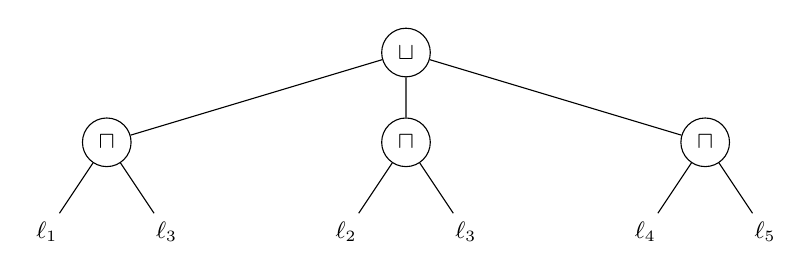
\begin{tikzpicture}[
  level distance=12mm,
  level 1/.style={sibling distance=40mm},
  level 2/.style={sibling distance=16mm},
  every node/.style={font=\small},
  op/.style={draw, circle, minimum size=6.5mm, inner sep=0.5mm},
  lit/.style={draw=none},
  scale=0.95, transform shape
]
\node[op] (root) {$\sqcup$}
  child { node[op] (cap1) {$\sqcap$}
    child { node[lit] {$\ell_1$} }
    child { node[lit] {$\ell_3$} }
  }
  child { node[op] (cap2) {$\sqcap$}
    child { node[lit] {$\ell_2$} }
    child { node[lit] {$\ell_3$} }
  }
  child { node[op] (cap3) {$\sqcap$}
    child { node[lit] {$\ell_4$} }
    child { node[lit] {$\ell_5$} }
  };
\end{tikzpicture}
\end{center}

\medskip
\noindent\textbf{\LUCO preservation.}
Comparing \LUCO relations before (as computed in Example~\ref{ex:AST}) and after normalization:
\begin{align*}
\LUCO_{\dnf(\phi)}(\ell_1,\ell_3) &= \sqcap \;=\; \LUCO_{\phi}(\ell_1,\ell_3),\\
\LUCO_{\dnf(\phi)}(\ell_2,\ell_3) &= \sqcap \;=\; \LUCO_{\phi}(\ell_2,\ell_3),\\
\LUCO_{\dnf(\phi)}(\ell_4,\ell_5) &= \sqcap \;=\; \LUCO_{\phi}(\ell_4,\ell_5),\\
\LUCO_{\dnf(\phi)}(\ell_1,\ell_2) &= \sqcup \;=\; \LUCO_{\phi}(\ell_1,\ell_2),\\
\LUCO_{\dnf(\phi)}(x,y) &= \sqcup \;=\; \LUCO_{\phi}(x,y)\quad
\text{for }x\in\{\ell_1,\ell_2,\ell_3\},\ y\in\{\ell_4,\ell_5\}.
\end{align*}
Thus, the \LUCO \emph{label} is preserved by $\dnf$, even though the \LUCO node may move,
e.g.\ $\ell_1,\ell_2$ are separated by the root $\sqcup$ in $\dnf(\phi)$.
\end{example}

when a formula has a punctual conflict any of its
equivalent formula satisfying \LUCO and
\LAP have a punctional conflict.








% \begin{lemma}[Preservation of Boolean operator alternation under $\pnf$]\label{lem:alternation}
% For any formula $\phi \in \TDDLfm$ and any bound $k \in \mathbb{N}$, the transformation $\pnf(\phi,k)$ preserves the syntactic alternation of Boolean operators in $\phi$.  
% In particular, the relative structure of conjunctions and disjunctions among sub-formulas of $\phi$ is unchanged in $\pnf(\phi,k)$.
% \end{lemma}
% \begin{proof}
% By Definition~\ref{def:pnf}, we have $\pnf(\phi,k)$ is homomorphic for conjunction in disjunction operators:\\
% $\pnf(\phi_1 \sqcap \phi_2,k)=  \pnf(\phi_1,k) \sqcap\pnf(\phi_2,k)$ \nd $\pnf(\phi_1 \sqcup \phi_2,k)=  \pnf(\phi_1,k) \sqcup \pnf(\phi_2,k)$.
% \end{proof}



% \begin{lemma}[Ancestor preservation of literals under $\pnf$]\label{lem:pnf-no-new-literals}
% For any $k\in\mathbb{N}$, every formula $\phi\in\TDDLfm$, and $\tool{D} \in \{\tool{O}, \tool{F}\}$, every literal $\monadop{D}{\is}{a}$ that occurs as a literal in $\pnf(\phi,k)$ has an ancestor literal $\monadop{D}{\is'}{a}$ that occurs in $\phi$ with $\is  \subseteq \bigcup \is'$.
% In particular, if $\is=\{[t,t]\}$ is punctual, then $t\subin \is'$.
% \end{lemma}


% \begin{proof}
% We proceed by structural induction on $\phi$, case-splitting according to Definition~\ref{def:pnf}.

% \emph{Base case (literal).}  
% If $\phi=\ob{\is}{a}$, then $\pnf(\phi,k)$ is either
% \[
% \bigsqcup_{t\in\is}\ob{\{[t,t]\}}{a}
% \]
% when $\max(\is)\le k$,  
% or
% \[
% \left(\bigsqcup_{t\in\is\ominus[k+1,\infty]}\ob{\{[t,t]\}}{a}\right)
% \sqcup \ob{\is\cap[k+1,\infty]}{a}
% \]
% when $\max(\is)>k$.  
% In both cases, every produced literal has the same modality and action as the original, and its interval set is included in $\is$.  
% The case $\phi=\forb{\is}{a}$ is analogous, using conjunction and the operators $\is\ominus[k+1,\infty]$ and $\is\cap[k+1,\infty]$.
% \emph{Inductive step.}  
% If $\phi=\phi_1\sqcap \phi_2$, then $\pnf(\phi,k)=\pnf(\phi_1,k)\sqcap \pnf(\phi_2,k)$; any literal in $\pnf(\phi,k)$ occurs in one of the sub-formula, and the induction hypothesis gives its ancestor in $\phi_1$ or $\phi_2$.  
% The case $\phi=\phi_1\sqcup \phi_2$ is identical.
% Thus, every literal in $\pnf(\phi,k)$ has an ancestor in $\phi$ with the same $(D, a)$ and an interval set covering all its points.  
% \end{proof}

% \begin{lemma}[Witness punctualization into $\pnf$]\label{lem:witness-punct-pnf}
% Let $\phi\in\TDDLfm$, when $k=\textsc{MaxOPoint}(\phi)$, and let
% $\ell_i=\monadop{Di}{\is_{i}}{a_i}$ and
% $\ell_j=\monadop{Dj}{\is_{j}}{a_j}$
% be literals that \emph{occur in} $\phi$ under a common conjunctive context.
% If there exists $t\in\mathbb{N}$ with $t\subin \is_i$ and $t\subin \is_j$ and $t\le k$,
% then $\pnf(\phi,k)$ contains punctual descendants
% \[
% \ell_i^p=\monadop{Di}{\{[t,t]\}}{a_i}
% \quad\text{and}\quad
% \ell_j^p=\monadop{Dj}{\{[t,t]\}}{a_j},
% \]
% each occurring at the respective literal positions (i.e., as descendants of
% $\ell_i$ and $\ell_j$) within the same conjunctive context inherited from $\phi$.
% \end{lemma}

% \begin{proof}
% By Definition~\ref{def:pnf}, each literal is refined \emph{in place}:
% obligations produce a disjunction over all $t\in  \is\cap\{[0,k]\}$ of
% $\ob{\{[t,t]\}}{a}$; prohibitions produce a conjunction over those $t$ of
% $\forb{\{[t,t]\}}{a}$. Thus $t\le k$ and $t\subin\is_i$ (resp.$\is_j$)
% imply that $\ell_i^p$ (resp.\ $\ell_j^p$) appears among the descendants of
% $\ell_i$ (resp.\ $\ell_j$). By the operator-skeleton preservation lemma for
% $\pnf$ (Lemma~\ref{lem:alternation}), the enclosing conjunction from
% $\phi$ remains at the same place in $\pnf(\phi,k)$, so both punctual descendants
% occur within that same conjunctive context. 
% \end{proof}

% We move now to study the same properties for the $\dnf$ normalization.

% \begin{lemma}[Preservation of Boolean operator alternation and literal ancestor relation under $\dnf$]
% \label{lemma:dnf-alt-anc}
% Let $\phi \in \TDDLfm$. Then the transformation $\dnf(\phi)$ satisfies the following properties:
% \begin{enumerate}[(i)]
%     \item \textbf{Boolean alternation preservation:} The syntactic alternation between conjunction and disjunction in $\phi$ is preserved in $\dnf(\phi)$ in the sense that every Boolean connective in $\dnf(\phi)$ has the same relative position (conjunctive or disjunctive level) as in some equivalent sub-formula of $\phi$.
%     \item \textbf{ancestor Literal preservation:} For every literal $\ell$ occurring in $\dnf(\phi)$, there exists a literal $\ell'$ occurring in $\phi$ such that $\ell$ is syntactically identical to $\ell'$.
% \end{enumerate}
% \end{lemma}

% \begin{proof}
% \emph{(i) Alternation preservation:}  
% We prove by contradiction. Assume there exists a sub-formula in $\dnf(\phi)$ whose Boolean operator alternation pattern differs from any alternation pattern in $\phi$. The only transformation used to obtain $\dnf(\phi)$ from $\phi$ is repeated application of the distributivity equivalences in Lemma~\ref{lemma:operequiv}, which replace a sub-formula of the form \\
% $\phi_1 \sqcap (\phi_2 \sqcup \phi_3)$ by $(\phi_1 \sqcap \phi_2) \sqcup (\phi_1 \sqcap \phi_3)$, or symmetrically for disjunction over conjunction. These rewritings do not invert the order of $\sqcap$ and $\sqcup$ but only propagate one operator outward. Thus, any alternation pattern in $\dnf(\phi)$ is inherited from some subformula of $\phi$, contradicting the assumption. Hence alternation is preserved.

% \emph{(ii) Ancestor preservation:}  
% Again, we proceed by contradiction. Suppose there exists a literal $\ell$ in $\dnf(\phi)$ such that no identical literal occurs in $\phi$. The $\dnf$ transformation rewrites only via distributivity and associativity, which neither introduces new literals nor modifies their deontic operator or time interval. Therefore, every literal in $\dnf(\phi)$ must have appeared unchanged in $\phi$. This contradicts the assumption, hence ancestor preservation holds.
% \end{proof}


\begin{theorem}[Soundness and Completeness of Algorithm~\ref{fig:conflict-extraction}]
\label{lem:conflict-sound-complete}
Let $\phi$ be any formula in \TDDLfm, and let $k=\textsc{MaxOPoint}(\phi)$.
Then Algorithm~\ref{fig:conflict-extraction} is sound and complete for detecting punctual conflicts in $\phi$: the set $\mathcall{PC}(\phi)$ returned by the algorithm contains \emph{exactly} the punctual conflicts specified by $\phi$.
\end{theorem}

\begin{proof}
We prove both directions\\
\smallskip\noindent
(I) Soundness:\\
Take any $(\pt,\mathcall{C})\in\mathcall{PC}(\phi)$ and any $\hat\ell\sqcap \hat\ell'\in\mathcall{C}$.
By definition of conflicts, $\hat\ell,\hat\ell'$ are punctual literals at a common time $t$ that match one
of \textbf{(P-Deon-Conf)} or \textbf{(P-Ont-Conf)}, and they co-occur in a product term of
$\dnf(\pnf(\phi,k))$.
By Lemma~\ref{lem:pnf-ancestor} (downward) each has an ancestor $\ell,\ell'$ in $\phi$
with the same modality/action and covering $t$. By Lemma~\ref{lem:pnf-luco} followed by
Lemma~\ref{lem:dnf-luco}, we have: (i), the \LUCO relating the two positions is preserved across
$\pnf$ and $\dnf$, since they are present conjunctively in the product term, the \LUCO in $\phi$
is $\sqcap$. Hence, $\ell\sqcap\ell'$ is a syntactically specified punctual pair in $\phi$,
of the same conflict type as $\hat\ell \sqcap \hat\ell'$ (types are syntactic and preserved).
Therefore, no product term forming a punctual conflict is introduced: every reported pair corresponds to one
already specified in $\phi$, and also its type(deontic vs ontic) is sound.

\smallskip\noindent
\emph{(II) Completeness.}  
\begin{enumerate}[(1)]
\item \textbf{All potential conflicts are exposed.}
Choose $k=\textsc{MaxOPoint}(\phi)$. Every time point relevant to \tool{O}/\tool{O} and
\tool{O}/\tool{F} conflicts is unfolded in $\pnf(\phi,k)$; prohibitions beyond $k$ cannot
yield punctual conflicts as there exists no conflict type involving two prohibitions. By Lemmas~\ref{lem:pnf-luco} and~\ref{lem:dnf-luco} (i), the \LUCO
for any literal pair is preserved through $\pnf$ and $\dnf$.

\item \textbf{All conflicts are localized and enumerated.}
If a conflict is specified in $\phi$ by a pair $\ell_i,\ell_j$ at some $t$ with
$\LUCO_\phi(\ell_i,\ell_j)=\sqcap$, then by Lemma~\ref{lem:witness-punct-pnf} there
exist punctual descendants at $t$ in $\pnf(\phi,k)$ under the same (conjunctive) \LUCO; by
Lemma~\ref{lem:dnf-luco} (ii) there is a product term of $\dnf(\pnf(\phi,k))$ containing both.
The algorithm checks \emph{every} pair in \emph{every} product term, ensuring that it catches them all.

\item \textbf{All conflict types are covered.}
By Lemma~\ref{lem:typeccomp}, punctual conflicts are exactly ontic or deontic.
The matching step of the algorithm recognizes precisely these patterns, so every possible punctual conflict is detected.
\end{enumerate}
By (I) and (II), we prove the correctness of the algorithm.
\end{proof}

After establishing the soundness and completeness of Algorithm~\ref{fig:conflict-extraction}, we analyze the cost of the full normalization chain that the algorithm relies on. The growth stems from two places: (i) \emph{punctual expansion} in $\pnf(\phi,k)$, which replaces each interval set by a boolean combination of punctual literals up to the bound $k$, and (ii) the \emph{cross-product} created when $\dnf$ distributes conjunctions over the disjunctions introduced by $\pnf$.

\begin{theorem}[Complexity of Full Normalization]\label{complexityofconf}
Let $\phi$ be a formula in \TDDLfm and let $k \in \mathbb{N}$ be a finite time bound. The transformation $\phi \to \dnf(\pnf(\phi,k))$ has worst-case space that is exponential in the average expansion factor of the interval sets in $\phi$ and the size of $\phi$.
\end{theorem}
\begin{proof}
We proceed in two stages, corresponding to the $\pnf$ and $\dnf$ transformations.

\textbf{Step 1: Punctual Normalization.}  
By Lemma~\ref{lem:pnf-size-expansion}, the size of the punctual normal form $\pnf(\phi,k)$ is bounded by a linear function of the original formula size and the average expansion factor of the interval sets:
\[
\pnf(\phi,k) \in \mathcall{O}\left( \expf_a(\phi) \cdot \size{\phi} \right).
\]
This step is therefore polynomial in $\size{\phi}$, assuming that $\expf_a(\phi)$ remains bounded.

\textbf{Step 2: Disjunctive Normalization.}  
By Lemma~\ref{lem:dnf}, every formula $\phi$ can be rewritten into an equivalent formula $\phi'$ in disjunctive normal form such that $\phi \dutyequiv \phi'$ and $\phi' := \bigsqcup_i \phi_i'$. However, the DNF transformation involves distributing conjunctions over disjunctions, which incurs an exponential increase in the number of product terms.

Each obligation literal $\ob{\is}{a}$ in $\pnf(\phi,k)$ generates a disjunction of size $\size{\is}$ (i.e., one punctual obligation per point), and each such disjunction contributes multiplicatively to the number of disjuncts in the DNF. Therefore, the number of product terms in $\dnf(\pnf(\phi,k))$ is at most exponential in the total number of punctual obligations introduced by $\pnf$, which is itself linear in $\expf_a(\phi) \cdot \size{\phi}$.

Thus, the total size of $\dnf(\pnf(\phi,k))$ is bounded by:
\[
\dnf(\pnf(\phi,k)) \in \mathcall{O}\left( 2^{\expf_a(\phi) \cdot \size{\phi}} \right),
\]
and so is the worst-case complexity of computing this transformation.
\end{proof}

We now prove the disjunctive modularity of our conflict detection algorithm.

\begin{lemma}[Conflict Extraction over Disjunctive Normal Form]
\label{lem:pc-dnf-union}
Let $\phi$ be a formula in \TDDLfm and let  $\phi':=\bigsqcup_{i=1}^n \phi_i'$ be the resulting formula from the disjunctive normalization obtained according to Lemma~\ref{lem:dnf}.
Then the set of tuples product term, conflicts obtained for $\phi$ is the union of the set of tuples product term, conflicts in its disjuncts:
$$
\mathcall{PC}(\phi) = \bigcup_{i=1}^n \mathcall{PC}(\phi_i').
$$
\end{lemma}

\begin{lemma}[Conflict extraction over disjunctive normal form]
\label{lem:pc-dnf-union}
Let $\phi\in\TDDLfm$ and let $\phi':=\bigsqcup_{i=1}^n \phi_i'$ be the disjunctive normal form of $\phi$ obtained according to Lemma~\ref{lem:dnf}. Then the set of (product–term, conflict–set) tuples returned by the extractor satisfies
\[
\mathcall{PC}(\phi)\;=\;\bigcup_{i=1}^n \mathcall{PC}(\phi_i').
\]
\end{lemma}

\begin{proof}
Recall what the extractor $\mathcall{PC}(\,\cdot\,)$ does (Algorithm~\ref{fig:conflict-extraction}): given an input
$\phi$, it computes $k=\textsc{MaxOPoint}(\phi)$, forms $\dnf(\pnf(\phi,k))$, and then, for
\emph{each} product term $\pt$ occurring at the top level of that DNF, it computes the set
$\mathcall{C}(\pt)$ of punctual conflicts by inspecting all pairs of literals in $\pt$ and
matching the fixed patterns \textbf{P-Deon-Conf} and \textbf{P-Ont-Conf}. It returns the set
$\{(\pt,\mathcall{C}(\pt)) \mid \mathcall{C}(\pt)\neq\emptyset\}$.

Let $k=\textsc{MaxOPoint}(\phi)$, and write $\phi'=\dnf(\pnf(\phi,k))=\bigsqcup_{i=1}^n \phi_i'$,
where each $\phi_i'$ is (by construction of DNF) a single product term (a conjunction of punctual literals).

We prove the stated equality by double inclusion.

\smallskip\noindent
$\subseteq$: Take any $(\pt,\mathcall{C})\in\mathcall{PC}(\phi)$. By the algorithm, $\pt$ is one of
the top-level product terms of $\phi'$, hence $\pt=\phi_j'$ for some $j\in\{1,\dots,n\}$. When the
extractor is run on $\phi_j'$ alone, the preprocessing is inert:
$\pnf(\phi_j',k)=\phi_j'$ (already punctual) and $\dnf(\phi_j')=\phi_j'$ (already a conjunction).
Therefore, the same per-term analysis over pairs of literals in $\pt$ is performed, yielding the
same conflict set $\mathcall{C}$. Hence $(\pt,\mathcall{C})\in\mathcall{PC}(\phi_j')\subseteq
\bigcup_{i=1}^n \mathcall{PC}(\phi_i')$.

\smallskip\noindent
$\supseteq$: Take any $(\pt,\mathcall{C})\in\mathcall{PC}(\phi_i')$ for some $i$. Since
$\phi_i'$ is a top-level product term of $\phi'$, the run of the extractor on $\phi$ will visit
that very product term $\pt=\phi_i'$ and execute the identical per-term scan, thus producing the
same $\mathcall{C}$. Therefore $(\pt,\mathcall{C})\in\mathcall{PC}(\phi)$.

\smallskip
In both directions, we used the following facts (i) DNF puts each product term at the top level, and (ii) the
conflict check is \emph{local} to each product term (it never compares literals across distinct
disjuncts). Hence $\mathcall{PC}(\phi)=\bigcup_{i=1}^n \mathcall{PC}(\phi_i')$.
\end{proof}

% \vspace{1em}
% \textbf{Notes:}
% \begin{itemize}
%     \item \texttt{maxtime point} extracts the largest time $t$ in obligation literals of $\phi$.
%     \item \texttt{pnf} and \texttt{dnf} are normalization functions preserving semantic equivalence.
%     \item \texttt{matchesConflictPattern} checks if conjunction $c$ matches known punctual conflicts such as \textbf{P-Deon-Conf} or \textbf{P-Ont-Conf}.
% \end{itemize}







\begin{example}[Conflict extraction on $\UC_1'$ and $\UC_2'$]\label{punctual conflicts detect}
We apply Algorithm~\ref{fig:conflict-extraction} to each disjunct of the normalized formula. 
$$
\UC' := \UC_1' \sqcup \UC_2'.
$$

\textbf{Step 1: Maximal Time Point.}  
The maximal time point in the obligation literals is $k = 16$.

\textbf{Step 2: Punctual Normal Form.}  
We apply the $\pnf$ up to point 16 to each formula:
\[
\begin{aligned}
\pnf(\UC_1',16) &= 
\left( \bigsqcup_{\substack{t \subin\\ \{[9,16]\}}} 
\ob{\{[t,t]\}}{\delAtGate} \right)  \sqcap \left( 
\bigsqcap_{\substack{t \subin\\ \{[2,4],[8,16]\}}} 
\forb{\{[t,t]\}}{\delAtGate} \sqcap 
\forb{\{[17,24]\}}{\delAtGate} \right)\\
&\quad \sqcap \left( \bigsqcap_{\substack{t \subin\\ \{[10,14]\}}} 
\forb{\{[t,t]\}}{\delAtPark} \right). \\
\pnf(\UC_2',16) &= 
\left( \bigsqcup_{\substack{t \subin\\ \{[9,16]\}}} 
\ob{\{[t,t]\}}{\delAtPark} \right) \sqcap \left( \bigsqcap_{\substack{t \subin\\ \{[10,14]\}}} 
\forb{\{[t,t]\}}{\delAtPark} \right) \\
& \quad \sqcap \left( 
\bigsqcap_{\substack{t \subin\\ \{[2,4],[8,16]\}}} 
\forb{\{[t,t]\}}{\delAtGate} \sqcap 
\forb{\{[17,24]\}}{\delAtGate} \right).
\end{aligned}
\]

\textbf{Step 3: Disjunctive Normal Form.}  
Distribute conjunction over disjunction to obtain \dnf. Each disjunct is formed by fixing one 
$t \subin \{[9,16]\}$ in the obligation disjunction.
\[\begin{array}{c}

				\dnf(\pnf(\UC_1',16))\\
				= \\
				\mathop{\bigsqcup}\limits_{\substack{t \subin\\ \{[9,16]\}}}
\left(
  \ob{\{[t,t]\}}{\delAtGate}
  \sqcap
  \mathop{\bigsqcap}\limits_{\substack{t' \subin\\ \{[10,14]\}}}
    \forb{\{[t',t']\}}{\delAtPark}
  \sqcap
  \mathop{\bigsqcap}\limits_{\substack{t'' \subin\\ \{[2,4],[8,16]\}}}
    \forb{\{[t'',t'']\}}{\delAtGate}
  \sqcap
  \forb{\{[17,24]\}}{\delAtGate}
\right)
\\
			\end{array}\]

and 
\[\begin{array}{c}

				\dnf(\pnf(\UC_2',16))\\
				= \\
				\mathop{\bigsqcup}\limits_{\substack{t \subin\\ \{[9,16]\}}}
\left(
  \ob{\{[t,t]\}}{\delAtPark}
  \sqcap
  \mathop{\bigsqcap}\limits_{\substack{t' \subin\\ \{[10,14]\}}}
    \forb{\{[t',t']\}}{\delAtPark}
  \sqcap
  \mathop{\bigsqcap}\limits_{\substack{t'' \subin\\ \{[2,4],[8,16]\}}}
    \forb{\{[t'',t'']\}}{\delAtGate}
  \sqcap
  \forb{\{[17,24]\}}{\delAtGate}
\right)
\\
			\end{array}\]



\textbf{Step 4: Conflict Detection.}  
The last step, which involves pattern matching conflicts, exhibits punctual conflicts $\UC_1'$. The punctual conflicts are of type deontic and are on product terms formed by the obligations on time points $10,11,12,13,\nd 14$ :
\[
\big\{
\ob{\{[t,t]\}}{\delAtGate} \sqcap \forb{\{[t,t]\}}{\delAtPark} \ \big| \ 
t \subin \{[10,14]\}
\big\}.\]

For $\UC_2'$, the algorithm detects deontic punctual conflicts in all product terms:
\[\
\big\{
\ob{\{[t,t]\}}{\delAtPark} \sqcap \forb{\{[t,t]\}}{\delAtPark} \ \big| \ 
t \subin \{[9,16]\}
\big\}.
\]
\end{example}









The example showcased two possible successful detections of punctual conflicts in two of the sub-formulas of our use case, namely $\UC_1' \nd \UC_2'$. Where $\UC_1'$ contained some conflicting product terms and $\UC_2'$ had punctual conflicts in all its product terms. We have also studied the satisfiability of the same sub-formulas in Example~\ref{satsolver}, and we have obtained that $\DC_1'$ is satisfiable and $\DC_2'$ is unsatisfiable.


We introduce the notion of \emph{conflict density} as a measure to quantify the prevalence of conflicts within normative specifications. High conflict density signals practical difficulty: it shrinks the set of specified feasible behaviors available to an agent, complicates compliance checking and planning, and blurs the specification's comprehensibility.  By formally capturing conflict density in  Def.~\ref{def:Conflict density-measure}, we provide a practical metric to guide the systematic refinement of normative specifications, supporting normative system designers in identifying and addressing overly restrictive or contradictory constraints.

\begin{definition}[Conflict Density]\label{def:Conflict density-measure}
Let $\phi$ be a formula from \TDDLfm and $k= \textsc{MaxOPoint}(\phi)$.  
We define the \defn{conflict density} for the formula $\phi$, written  $\cd(\phi)$, as the ration between the conflicting product terms and  the total number of product terms in $\dnf(\pnf(\phi,k))$, formally:
$$
\cd(\phi) := \frac{\size{\mathcall{PC}(\phi)}}{\Xi(\phi)} \quad.
$$
Where:
\begin{itemize}
    \item $\size{\mathcall{PC}(\phi)}$ is the cardinality of the set of pairs returned by  Algorithm~\ref{fig:conflict-extraction} on $\phi$, and
    \item $\Xi(\phi)$ is \defn{the number of product terms} in $\dnf(\pnf(\phi,k))$.
\end{itemize}
\end{definition}
The conflict density $\cd(\phi)$ captures the proportion of conflicting punctual obligations  that are involved in conflicts, providing an indicator of how overloaded the normative specification is, that is, the fraction of time points where an obligation is prescribed but cannot actually be fulfilled. When $\cd(\phi)=0$ we say that $\phi$ is \defn{conflict free}, and $\phi$ is said to be \defn{fully conflicting} when $\cd(\phi)=1$.

\begin{example}[Conflict density measure computation]
We now compute the conflict density measure $\cd(\phi)$ based on the analysis done for Example~\ref{ex:easy}.

From Table~\ref{table:conflict-analysis}, we know that:
\begin{itemize}
    \item The number of product terms in $\dnf(\pnf(\phi,2))$ is $\Xi(\phi) = 4$,
    \item The number of product terms containing at least one punctual conflict  is $\size{\mathcall{PC}(\phi)} = 3$.
\end{itemize}

Hence, by Definition~\ref{def:Conflict density-measure}, we compute the conflict density measure as:
$$
\cd(\phi) = \frac{3}{4} = 0.75.
$$
This conflict density value indicates a high level of conflict density, as 75\% of the product terms are involved in conflicts, either deontic or ontic. In practice, such a high conflict density may suggest  overloaded normative constraints in the normative specification.
\end{example}


\begin{example}[Computing conflict density measure for $\UC_1'$ and $\UC_2'$]\label{ex:Conflict density-UC1-UC2}
Building on Example~\ref{punctual conflicts detect}, we compute the Conflict density measure for the disjuncts $\UC_1'$ and $\UC_2'$ individually.

\textbf{Step 1: Conflict Count.}  
From the conflict detection phase, we have clauses containing exactly one conflict per clause:
\[
\mathcall{PC}(\UC_1') = 
\big\{
\ob{\{[t,t]\}}{\delAtGate} \sqcap \forb{\{[t,t]\}}{\delAtGate} \sqcap \forb{\{[2,4],[8,24]\}}{\delAtPark} \ \big| \ t \subin \{[10,14]\}
\big\}, \quad \text{so } \size{\mathcall{PC}(\UC_1')} = 5.
\]

\[
\mathcall{PC}(\UC_2') = 
\big\{
\ob{\{[t,t]\}}{\delAtPark} \sqcap \forb{\{[t,t]\}}{\delAtPark} \ \big| \ t \subin \{[9,16]\}
\big\}, \quad \text{so } \size{\mathcall{PC}(\UC_2')} = 8.
\]

\textbf{Step 2: Obligation Count.}  
From the Punctual Normal Form \pnf up to 16 we know:
\[
\UC_1' \text{ generates } 8 \text{ punctual obligations on } \delAtGate \quad (t \subin \{[9,16]\}),
\]
\[
\UC_2' \text{ generates } 8 \text{ punctual obligations on } \delAtPark \quad (t \subin \{[9,16]\}).
\]

\textbf{Step 3: Conflict density Measures.}
\[
\cd(\UC_1') = \frac{\size{\mathcall{PC}(\UC_1')}}{\Xi(\UC_1')} = \frac{5}{8} = 0.625,
\]
\[
\cd(\UC_2') = \frac{\size{\mathcall{PC}(\UC_2')}}{\Xi(\UC_2')} = \frac{8}{8} = 1.
\]


$\UC_2'$ has conflict density of 1, with every punctual obligation point involved in a conflict.  
$\UC_1'$ has a conflict density less than 1, with conflicts at five of the eight obligation points.

We move now to do it for the overall use case we have, following Lemma~\ref{lem:pc-dnf-union}: \[
\mathcall{PC}(\UC) = \mathcall{PC}(\UC_1') \cup \mathcall{PC}(\UC_2').
\]

With:
\[
\size{\mathcall{PC}(\UC_1')} = 5 \quad \text{and} \quad \size{\mathcall{PC}(\UC_2')} = 8.
\]
So:
\[
\size{\mathcall{PC}(\UC)} = 13.
\]

\textbf{Obligation count.}  
From the punctual normal form construction:
\[
\UC_1' \text{ and } \UC_2' \text{ each produce } 8 \text{ punctual obligations }( 1 \text{ per } t \subin \{[9,16]\}).
\]
Thus:
\[
\Xi(\UC) = 16.
\]

\textbf{Conflict density measure.}  
Applying the definition:
\[
\cd(\UC) = \frac{\size{\mathcall{PC}(\UC)}}{\Xi(\UC)} = \frac{13}{16} \approx 0.8125.
\]
This indicates that approximately 81\% of punctual obligation points in $\UC$ are involved in conflicts and thus cannot be used to comply with the normative system.
\end{example}

We proceed to study the relationship between the unsatisfiability of a formula and its conflict density.
\begin{lemma}[Fully conflicting means Unsatisfiable]
\label{lem:full-Conflict density-unsat}
Let $\phi$ be a formula in \TDDLfm. Then $\phi$ is fully conflicting, i.e., $\cd(\phi) = 1$, if and only if $\phi$ is unsatisfiable.
\end{lemma}


\begin{proof}
($\Rightarrow$) Assume $\cd(\phi) = 1$.  
By Definition~\ref{def:Conflict density-measure}, we have:
$$
\frac{\size{\mathcall{PC}(\phi)}}{\Xi(\phi)} = 1.
$$
This implies that every punctual obligation literal generated by $\pnf(\phi,k)$ participates in a punctual conflict. In the \dnf expansion of $\pnf(\phi)$, each product term includes at least one such obligation, and by definition of punctual conflict, this yields an unsatisfiable conjunction by conjunction extension. Since all product terms are unsatisfiable, their disjunction is unsatisfiable. Hence, $\phi$ is unsatisfiable.

($\Leftarrow$) Now assume $\phi$ is unsatisfiable.  
By Lemma~\ref{lem:pc-dnf-union}, the set of punctual conflicts $\mathcall{PC}(\phi)$ is the union of the punctual conflicts found in each \dnf disjunct. If $\phi$ is unsatisfiable, there exists no word satisfying the formula. Then every product term in $\dnf(\pnf(\phi, k))$ must also be unsatisfiable, so each contains a punctual conflict. Moreover, since an unsatisfiable formula must have all its obligation points involved in conflict (otherwise at least one satisfying assignment would exist for a disjunct), it follows that:
$$
\size{\mathcall{PC}(\phi)} = \Xi(\phi),
$$
and hence $\cd(\phi) = 1$.

Therefore, $\phi$ is fully conflicting if and only if it is unsatisfiable.
\end{proof}


\begin{theorem}[Conflict free pruning for Partially conflicting Formulas]
\label{thm:pruning-partial-Conflict density}
Let $\phi\in\TDDLfm$ with $\cd(\phi)\neq 1$ (i.e., $\phi$ is not fully conflicting). 
Then there exists a formula $\phi'$ such that
\[
\phi \equiv \phi' \quad\text{and}\quad \cd(\phi')=0.
\]
\end{theorem}

\begin{proof}[Proof (by constructive pruning via Algorithm~\ref{fig:conflict-extraction})]
Let $k=\textsc{MaxOPoint}(\phi)$ and build 
\[
\phi_{\text{dpnf}} \ :=\ \dnf(\pnf(\phi,k)) \ =\ \bigsqcup_{i=1}^{n}\pt_i,
\]
where each $\pt_i$ is a product term (conjunction of punctual literals).

Run Algorithm~\ref{fig:conflict-extraction} on $\phi$ and obtain
\[
\mathcall{PC}(\phi)\ =\ \{\,(\pt_i,\mathcall{C}_{\pt_i})\ :\ 1\le i\le n,\ \mathcall{C}_{\pt_i}\neq\emptyset\,\}.
\]
By definition of $\cd$ (Definition~\ref{def:Conflict density-measure}), $\cd(\phi)\neq 1$ implies that \emph{not all} product terms are conflicting, i.e., the index set formed by non-conflicting product terms
$
I\ :=\ \{\, i\in\{1,\dots,n\} \mid \mathcall{C}_{\pt_i}=\emptyset \,\}$ is nonempty.

Define the pruned disjunction
\[
\phi' \ :=\ \bigsqcup_{i\in I}\ \pt_i.
\]

\emph{Equivalence.}
By Lemma~\ref{lem:dpnf-semantics}, $\phi\equiv \phi_{\text{dpnf}}$.
For every $j\notin I$, Algorithm~\ref{fig:conflict-extraction} returned a nonempty conflict set $\mathcall{C}_{\pt_j}\neq\emptyset$, meaning $\pt_j$ contains a punctual conflict. By the definition of punctual conflict and closure under conjunction, each such $\pt_j$ is unsatisfiable. Hence,
\[
\phi_{\text{dpnf}}\ \equiv\ \Big(\bigsqcup_{i\in I}\pt_i\Big)\ \sqcup\ \Big(\bigsqcup_{j\notin I}\underbrace{\pt_j}_{\bot}\Big)\ \equiv\ \bigsqcup_{i\in I}\pt_i\ =\ \phi'.
\]
Therefore $\phi\equiv \phi'$.

\emph{Zero conflict density.}
By construction, every disjunct $\pt_i$ retained in $\phi'$ satisfies $\mathcall{C}_{\pt_i}=\emptyset$. Thus $\mathcall{PC}(\phi')=\emptyset$ and, by Def.~\ref{def:Conflict density-measure}, $\cd(\phi')=0$.

This completes the constructive proof: $\phi'$ is obtained by (i) computing $\pnf$ and $\dnf$, (ii) calling Algorithm~\ref{fig:conflict-extraction} to mark conflicting product terms, and (iii) Put into the disjunction only the conflict-free ones.
\end{proof}

Having established that Algorithm~\ref{fig:conflict-extraction} is sound and complete for detecting punctual conflicts, we now turn to the question of how to refine a formula by \emph{eliminating} such conflicts. The idea is to discard any product term in the disjunctive punctual normal form that contains a conflict, thereby retaining only those disjuncts that remain consistent. This yields a conflict-free rewriting of the input formula, which we denote by $\Namb(\phi)$. By construction and by Theorem~\ref{lem:conflict-sound-complete}, every conflict identified and removed in this process corresponds to a genuine conflict specified by $\phi$, ensuring the soundness of the refinement. Formally, a variant of this algorithm would consist of: if every product term of $\dnf(\pnf(\phi,k))$ contains a punctual conflict, then no refinement is possible and the procedure returns \textbf{False}. Otherwise, $\Namb(\phi)$ is defined as the disjunction of all conflict-free product terms. The construction is given in Algorithm~\ref{alg:conflict-free-rewriting}.




\begin{minipage}{0.95\textwidth}
    \center{
\begin{algorithm}[H]
\caption{Procedure \textsc{Conflict-Free Rewriting} \Namb}
\label{alg:conflict-free-rewriting}
\KwIn{A formula $\phi \in \TDDLfm$}
\KwOut{\textbf{False} if every product term contains a punctual conflict; else a conflict-free refined formula $\Namb(\phi)$}

\BlankLine
$k \gets \textsc{MaxOPoint}(\phi)$ \tcp*{Largest obligation time point in $\phi$}

$\phi_{\mathrm{pnf}} \gets \pnf(\phi, k)$ \tcp*{Punctual normal form up to $k$}

$\phi_{\mathrm{dnf}} \gets \dnf(\phi_{\mathrm{pnf}})$ \tcp*{Convert to disjunctive normal form}

$\CF(\phi) \gets \emptyset$ \tcp*{Will collect non-conflicting product terms}

\ForEach{product term $\pt$ in $\phi_{\mathrm{dnf}}$}{
  $\textit{hasConflict} \gets \textbf{false}$\;
  \ForEach{pair of literals $(\ell_1,\ell_2)$ in $\pt$}{
    \If{$(\ell_1,\ell_2)$ matches \textbf{P-Deon-Conf} or \textbf{P-Ont-Conf}}{
      $\textit{hasConflict} \gets \textbf{true}$\;
      \textbf{break} \tcp*{No need to inspect more pairs in this $\pt$}
    }
  }
  \If{\textbf{not} $\textit{hasConflict}$}{
    $\CF(\phi) \gets \CF(\phi) \cup \{\pt\}$ \tcp*{Keep $\pt$: it is conflict-free}
  }
}

\If{$\CF(\phi)=\emptyset$}{
  \Return \textbf{False} \tcp*{All disjuncts have conflicts}
}
$\Namb(\phi) \gets \displaystyle\bigsqcup_{\pt \in \CF(\phi)} \pt$ \tcp*{Rebuild from conflict-free terms}
\Return $\Namb(\phi)$

\end{algorithm}}
\end{minipage}

\begin{remark}
    An optimized variant of Algorithm~\ref{alg:conflict-free-rewriting} can be obtained by incorporating an early satisfiability check. Before initiating the normalization and conflict-removal procedure, we first test whether the input formula $\phi$ is unsatisfiable, for instance using \textsc{checksat}$(\phi)$. If the result is negative, the procedure immediately returns \textbf{False}, since no conflict-free refinement can exist. This optimization avoids the potentially expensive construction of the punctual and disjunctive normal forms in cases where the formula is already inconsistent at the semantic level.
\end{remark}


The constructive pruning proof above does more than guarantee existence: it \emph{computes} the conflict-free disjuncts explicitly. Each conflict-free product term can be read as an executable policy clause. The next remark makes this operational connection precise.

\begin{remark}[Relation to planning]
Our pruning view is closely related to model enumeration (All-SAT), a standard task in SAT/SMT and Constraint Satisfaction Problem (CSP) as in ~\cite{valiant1979complexity,gomes2008model,creignou2011enumerating}. After removing all conflicting product terms from the \dpnf, what remains is a precisely delimited set of conforming, norm-following paths that a planner can safely execute. Each remaining disjunct specifies a consistent set of time-stamped obligations and prohibitions, i.e., a feasible and normatively compliant policy fragment.

A practical strategy is: (i) within a chosen product term, merge all prohibitions on the same action into a single prohibition interval set so that only punctual obligations remain as clear action points; and (ii) execute exactly those obligations at their designated time points while abstaining from all prohibited actions. This reduces planning to selecting one conflict-free clause, reading off its obligation timestamps, and committing to those actions. The choice is also explainable, e.g., “We selected product term~2, so we act at times $\{t_1,t_2,\dots\}$ and avoid all other actions by construction.”
\end{remark}

\noindent Having framed conflict elimination as a generator of clear, compliant planning options, we now turn to an orthogonal concern: the \emph{conciseness} of the resulting representation. Although our analysis detects and removes conflicts, the intermediate normalizations (\pnf and \dnf) can dramatically increase syntactic size. In the next subsection, we discuss this blow-up.


\subsection{Induced Verbosity from Eliminating Punctual Conflicts}\label{induced verbosity}

Eliminating punctual ontic conflicts yields conflict free formulas, but it can substantially increase syntactic size. The source of this blow-up is combinatorial: to respect the “at most one action per time point” assumption, one may enumerate only those product terms whose punctual obligations are scheduled at pairwise distinct times.


\begin{example}
\[
\phi \;:=\; \ob{\{[0,3]\}}{\mathsf{a}} \ \sqcap\  \ob{\{[0,3]\}}{\mathsf{b}} \ \sqcap\  \ob{\{[0,3]\}}{\mathsf{c}}.
\]
All three obligation literals share the same interval set and are conjoined, so at each $t\in\{0,1,2,3\}$ the pairwise $\tool{O}$–$\tool{O}$ combinations (e.g., $\ob{\{[t,t]\}}{\mathsf{a}}\sqcap\ob{\{[t,t]\}}{\mathsf{b}}$) yield punctual ontic conflicts.

Table~\ref{table:ontic-triple-conflict} shows the transformation pipeline: \pnf, \dnf, conflict extraction, and the construction of a conflict free rewriting $\Namb(\phi)$ that prunes all conflicting product terms. As the last row indicates, $\Namb(\phi)$ is about $20\times$ larger than the original $\phi$ under our size metric.

Intuitively, $\dnf(\pnf(\phi,3))$ enumerates all $4^3$ assignments of times to $(\mathsf{a},\mathsf{b},\mathsf{c})$. To avoid ontic conflicts, we must keep only those assignments where the three times are \emph{pairwise distinct}, i.e., $4\cdot3\cdot2=24$ product terms. This necessary filtering still yields a sizeable disjunction.

\begin{table}[h]
\centering
\renewcommand{\arraystretch}{1.5}
\begin{tabular}{|l|p{8cm}|c|}
\hline
\textbf{Step} & \textbf{Expression} & \textbf{Size} \\
\hline
$\phi$ 
& 
$\ob{\{[0,3]\}}{\mathsf{a}} \ \sqcap\  \ob{\{[0,3]\}}{\mathsf{b}} \ \sqcap\  \ob{\{[0,3]\}}{\mathsf{c}}$
& 18 \\
\hline
$\pnf(\phi,3)$ 
& 
$\Big( \bigsqcup_{i=0}^{3} \ob{\{[i,i]\}}{\mathsf{a}} \Big)
\ \sqcap\
\Big( \bigsqcup_{i=0}^{3} \ob{\{[i,i]\}}{\mathsf{b}} \Big)
\ \sqcap\
\Big( \bigsqcup_{i=0}^{3} \ob{\{[i,i]\}}{\mathsf{c}} \Big)$
& 59 \\
\hline
$\dnf(\pnf(\phi,3))$ 
& 
$\displaystyle
\bigsqcup_{\substack{0 \leq i,j,k \leq 3}} 
\Big( \ob{\{[i,i]\}}{\mathsf{a}} \ \sqcap\  \ob{\{[j,j]\}}{\mathsf{b}} \ \sqcap\  \ob{\{[k,k]\}}{\mathsf{c}} \Big)
$
& 959 \\
\hline
Punctual conflicts 
& 
$\displaystyle
\big\{
\ob{\{[t,t]\}}{\mathsf{a}} \sqcap \ob{\{[t,t]\}}{\mathsf{b}},\
\ob{\{[t,t]\}}{\mathsf{a}} \sqcap \ob{\{[t,t]\}}{\mathsf{c}},$
& -- \\
in $\mathcall{PC}(\phi)$ &$
\ob{\{[t,t]\}}{\mathsf{b}} \sqcap \ob{\{[t,t]\}}{\mathsf{c}}
\ \big|\ t\in\{0,1,2,3\}
\big\}
$ &
\\
\hline
$\Namb(\phi)$
& 
$\displaystyle
\bigsqcup_{\substack{i,j,k \in \{0,1,2,3\}\\ \text{pairwise distinct}}}
\Big( \ob{\{[i,i]\}}{\mathsf{a}} \ \sqcap\  \ob{\{[j,j]\}}{\mathsf{b}} \ \sqcap\  \ob{\{[k,k]\}}{\mathsf{c}} \Big)
$
& 359 \\
\hline
$\displaystyle \frac{\size{\Namb(\phi)}}{\size{\phi}}$ 
& 
Conflict elimination blow-up factor 
& $\approx 20$ \\
\hline
\end{tabular}
\caption{Conflict elimination size comparison for $\phi := \ob{\{[0,3]\}}{\mathsf{a}} \sqcap \ob{\{[0,3]\}}{\mathsf{b}} \sqcap \ob{\{[0,3]\}}{\mathsf{c}}$.}
\label{table:ontic-triple-conflict}
\end{table}
\end{example}

While the worst case can be large, a conflict free rewrting of a formula often admits a more concise equivalent by \emph{merging} punctual literals on the same action. In particular, disjunctions of punctual obligations on the same action can be compressed by \textbf{ObDis}, and conjunctions of punctual prohibitions can be compressed by \textbf{FConj}.

\begin{example}
Consider
\[
\UC_2' \;:=\; \ob{\{[9,16]\}}{\delAtPark} \ \sqcap\  \forb{\{[10,14]\}}{\delAtPark} \ \sqcap\  \forb{\{[2,4],[8,24]\}}{\delAtGate}.
\]
The conflict free rewriting $\Namb(\UC_2')$ prunes all conflicting product terms, leaving exactly the non-conflicting obligation times $t\in\{9,15,16\}$. A literal (still verbose) form is:
\begin{table}[h] \centering \renewcommand{\arraystretch}{1.5} \begin{tabular}{|l|p{10.5cm}|c|} \hline \textbf{Formula} & \textbf{Expression} & \textbf{Size} \\ \hline $\UC_2'$ & $\ob{\{[9,16]\}}{\delAtPark} \sqcap \forb{\{[10,14]\}}{\delAtPark} \sqcap \forb{\{[2,4], [8,24]\}}{\delAtGate}$ & 16 \\ \hline
     $\Namb(\UC_2')$ & $ \left(
        \ob{\{[9,9]\}}{\delAtPark}
        \sqcup
        \ob{\{[15,15]\}}{\delAtPark}
        \sqcup
        \ob{\{[16,16]\}}{\delAtPark}
      \right)
      \sqcap
      \mathop{\bigsqcap}\limits_{t \in [10,14]}
      \forb{\{[t,t]\}}{\delAtPark}
      \sqcap
        \forb{\{[2,4],[8,24]\}}{a} $ & 94 \\ 
     \hline $\UC_2''$ & $\ob{\{[9,9], [15,16]\}}{\delAtPark} \sqcap \forb{\{[10,14]\}}{\delAtPark} \sqcap \forb{\{[2,4], [8,24]\}}{\delAtGate}$ & 18 \\ \hline \end{tabular} \caption{Refactoring a verbose conflict free rewriting $\Namb(\UC_2')$ into a more concise equivalent $\UC_2''$.} \label{table:refactoring-uc2} \end{table}
Here $\UC_2''$ compresses the three surviving punctual obligations on \delAtPark\ into a single obligation over $\{[9,9],[15,16]\}$, while prohibitions on \delAtGate\ are merged back into their original interval sets.
\end{example}

These examples motivate \emph{controlled} conflict density management: when readability/size matters, designers can (i) keep compact high-level formulas that \emph{implicitly} contain ontic conflicts and resolve them later during planning, or (ii) eliminate conflicts upfront and then refactor the resulting \dpnf\ with merging rules (\textbf{ObDis}, \textbf{FConj}) to restore conciseness. In the next section, we present a generalized conflict rule over punctual literals that unifies deontic and ontic cases and supports concise rewriting without fully enumerating the \dpnf.

\subsection{Generalized Conflict Rules and Conflict Calculus}\label{subsec:calculus}
The previous section demonstrated that eliminating punctual conflicts may lead to significant increases in formula size. While some verbose conflict free rewriting formulas can be refactored into more concise forms, this is not always possible without losing semantic precision. In this section, we generalize the conflict scenarios observed earlier and formalize them as inference rules. These rules allow the user to explore the formula and choose which conflicts to remove.


We define in Table~\ref{syncnotation} syntactic notations build upon the extensional semantics from our logical framework to express rules for our deductive conflict analysis system. It introduces derivations such as entailment ($\vdash$) and equivalence ($\equiv$). Notice that if $\phi \vdash \phi'$ and $\phi' \vdash \phi$ then $\phi \equiv \phi'$ and $\phi' \equiv \phi$:
 \begin{itemize}
 \item We denote by $\phi \dutymodel \bot$ that the formula $\phi$ is inconsistent in our reasoning, i.e., it is unsatisfiable, so $\dutyclass{\phi} = \emptyset$. 
\item We denote by $\dutymodel \phi$ that the formula $\phi$ is valid in our proof system, we map it to its satisfiability by any possible \timedword, i.e., $\dutyclass{\phi} = 2^\domtr$.    
\item We denote by $\phi\dutymodel \phi'$ that formula $\phi$ entails $\phi'$, which holds when $\dutyclass{\phi} \subseteq \dutyclass{\phi'}$.   
\item Equivalence is written as $\phi \dutyequiv \phi$, which holds when $\dutyclass{\phi} = \dutyclass{\phi'}$. 
\end{itemize}

\begin{table}[h]
    \centering
    \begin{tabular}{|c|c|c|}
      \hline
      \emph{Notation} & \emph{Signification} & \emph{Semantic mapping} \\ \hline
      $\phi \vdash \bot$ 
        & $\phi$ is inconsistent 
        & $\dutyclass{\phi} = \emptyset$ \\ \hline
      $\vdash \phi$ 
        & $\phi$ is valid 
        & $\dutyclass{\phi} = 2^{\domtr}$ \\ \hline
      $\phi \vdash \phi'$ 
        & $\phi$ entails $\phi'$ 
        & $\dutyclass{\phi} \subseteq \dutyclass{\phi'}$ \\ \hline
      $\phi \equiv \phi'$ 
        & $\phi$ is equivalent to $\phi'$ 
        & $\dutyclass{\phi} = \dutyclass{\phi'}$ \\ \hline
    \end{tabular}
    \caption{Syntactic notations and their semantic mapping}
    \label{syncnotation}
  \end{table}